%%%%%%%%%%%%%%%%%%%%%%%%%%%%%%%%%%%%
\chapter{Results}

This section gives the results of the primary tasks of this thesis: the classification of jobs according to whether or not they include environmental activities, described in Section~\ref{chap:procedure}, and the association of jobs to activities and skills, the procedure of which is outlined in Section~\ref{sec:activites}.

The full results for all 8565 jobs in the data set can be found in the Results folder of the repository in Ref~\cite{emilysharata}. Only a small labeled data set is available for the categorization task. For the association of jobs to skills, the performance is assessed by manually inspecting a small, random subset of the results. Additional labeling and inspection of the results is possible on the full data set, which is made available, but is outside the scope of the present discussion.
\label{chap:Results}
%%%%%%%%%%%%%%%%%%%%%%%%%%%%%%%%%%%%
\section{Environmental job classification}
\label{sec:greenresults}

To have an understanding of a baseline neural network performance for this particular classification task, inspection of the confusion matrix of the simpler neural network model described in  is used. This model uses the Adam adaptive learning rate method and three epochs. The confusion matrix is shown in Fig~\ref{fig:simpleModelConfusion}. The F-measure for this model is 0.785.


\begin{figure}[htbp]
  \centering
    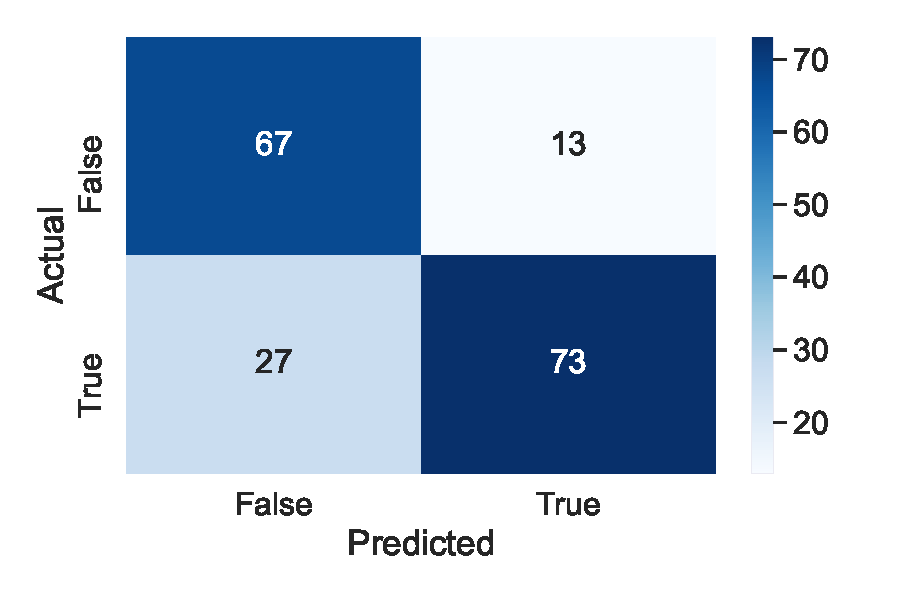
\includegraphics[width=0.5\textwidth]{figures/simpleModelConfusion.pdf}
    \caption{
    	The confusion matrix of the simpler neural network model, using 3 epochs and the Adam optimizer. 
    	}
\label{fig:simpleModelConfusion}
\end{figure}

The more complex neural network model is then optimized by changing the adaptive learning rate method and the number of epochs. Four different combinations are evaluated: The Adam optimizer with three epochs (Fig~\ref{fig:Complex3Adam}), the Adam optimizer with six epochs (Fig~\ref{fig:Complex6Adam}), the RMS Prop optimizer with three epochs (Fig~\ref{fig:Complex3RMSProp}), and the RMS Prop optimizer with six epochs (Fig~\ref{fig:Complex6RMSProp}). The 

The Adam and RMS Prop optimizers produce similar results, although the number of true negatives 

\begin{figure}[htbp]
  \centering
    \includegraphics[width=0.5\textwidth]{figures/Complex3Adam.pdf}
    \caption{
    	The confusion matrix of the more complex neural network model, using 3 epochs and the Adam optimizer. The F-measure for this model is 0.799.
    	}
\label{fig:Complex3Adam}
\end{figure}

\begin{figure}[htbp]
  \centering
    \includegraphics[width=0.5\textwidth]{figures/Complex6Adam.pdf}
    \caption{
    	The confusion matrix of the more complex neural network model, using 6 epochs and the Adam optimizer. The F-measure for this model is 0.800.
    	}
\label{fig:Complex6Adam}
\end{figure}

\begin{figure}[htbp]
  \centering
    \includegraphics[width=0.5\textwidth]{figures/Complex3RMSProp.pdf}
    \caption{
    	The confusion matrix of the more complex neural network model, using 3 epochs and the RMS Prop optimizer. The F-measure is 0.803.
    	}
\label{fig:Complex3RMSProp}
\end{figure}

\begin{figure}[htbp]
  \centering
    \includegraphics[width=0.5\textwidth]{figures/Complex6RMSProp.pdf}
    \caption{
    	The confusion matrix of the more complex neural network model, using 6 epochs and the RMS Prop optimizer. The F-measure is 0.801.
    	}
\label{fig:Complex6RMSProp}
\end{figure}


Although all very similar in performance, the model with the highest F-measure is the more complex model using three epochs and the RMS Prop optimizer. With an F-measure of 0.801, it slightly outperforms the other models.


\section{Job skill and activity association}
\label{sec:activityresults}

In order to identify the relevant skills and activities in the job offers text, the cosine distance cutoffs found and discussed in Section~\ref{sec:activites} are used. Using the cosine distance cutoff of 0.8491, the number of activity matches can be compared to the top 10 activity matches by distance. Fig.~\ref{fig:AllActMatches13763695} shows the top 10 activity matches to the job offer 13763695. Fig.~\ref{fig:GoodActMatches13763695} shows the activity matches to the job offer 13763695 using the cosine distance cutoff. Certain activities in the the diagram showing the top 10 best matched activities are clearly irrelevant to the job offer. For example, ``apply protective coatings,'' is not contained in the text although it is the 10th most semantically similar sentence to the sentences in the job offer. 

\begin{figure}[htbp]
  \centering
    \includegraphics[width=1.0\textwidth]{figures/AllActMatches13763695.pdf}
    \caption[The top 10 activity matches to the job offer 13763695]{
    The top 10 activity matches to the job offer 13763695. The content of the job offer is shown on the left, and the activity matches are shown on the right. 
    }
\label{fig:AllActMatches13763695}
\end{figure}

\begin{figure}[htbp]
  \centering
    \includegraphics[width=1.0\textwidth]{figures/GoodActMatches13763695.pdf}
    \caption[The activity matches to the job offer 13763695 using the cosine distance cutoff of 0.8491]{
    The activity matches to the job offer 13763695 using the cosine distance cutoff of 0.8491. The activity matches are shown on the left, and the content of the job offer is shown on the right. 
    }
\label{fig:GoodActMatches13763695}
\end{figure}

For the skills, the same comparison is made between the top ten matches by distance and the skills matches with the cosine cutoff distance of 0.8158. Fig.~\ref{fig:GoodSkillMatches} shows the top ten skills matches for job offer 13763695. In this particular case, the top ten best matched skills are all within the 0.8158 cutoff, as the matches are exactly the same. The is not an unusual result, as there can be many skills that can be legitimately applicable to each job offer. 

\begin{figure}[htbp]
  \centering
    \includegraphics[width=1.0\textwidth]{figures/GoodSkillMatches.pdf}
    \caption[The skill matches to the job offer 13763695 using the cosine distance cutoff of 0.8158]{
    The skill matches to the job offer 13763695 using the cosine distance cutoff of 0.8158. The activity matches are shown on the right, and the content of the job offer is show on the left. 
    }
\label{fig:GoodSkillMatches}
\end{figure}

With a visual inspection, it is clear that many of these matched skills and activities are indeed relevant, especially the top one or two matches (i.e., those with the lowest cosine similarity scores, shown at the beginning of the listed skills). However, there still exists some room for matching refinement. For example, the activity match ``performing day-to-day administrative tasks such as maintaining information files and processing paperwork'' is best matched with the sentence from the sentences in the job offer `do not hesitate to send your full application file with motivation file' and 'curriculum vitae copies of diplomas and work certificates via Jobup only.' In this case, these sentences inn the job offer are only referring to the application procedure, and not the functions of the job itself. Therefore, in future research it will be necessary to either further experiment with the cutoff cosine distances, or perhaps more practically, develop a method to remove the irrelevant parts of the job offers text. The full results of the relative skills and activities identification can be found 
